
\documentclass[twocolumn,cm]{article}
\usepackage[top=0.5in, left=0.45in, right=0.45in, bottom=0.5in]{geometry}

\usepackage{url}
\usepackage{code}
% \usepackage{cite}
\usepackage{amsmath}
\usepackage{amssymb}
\usepackage{graphicx}

\usepackage{nopageno}

\interfootnotelinepenalty=0

% lets me explicitly set a. or 1. etc. as enum label
\usepackage{enumitem}

\pagestyle{empty}

\usepackage{ulem}
% go back to italics for emphasis, though
\normalem

\usepackage{natbib}

\setlength{\footnotesep}{2em}

\newcommand\comment[1]{}
\newcommand\sfrac[2]{\!{}\,^{#1}\!/{}\!_{#2}}

\newcommand\nan{\textsf{NaN}}
\renewcommand\inf{\textsf{inf}}

\newcommand\plusminus{\pm}

\begin{document} 

\newcommand\ieee[2]{[{\it IEEE 754-2008}, #1, p#2]}

% flInf flops?
\title{NaN gates and flip FLOPS}
\author{Dr.~Tom~Murphy~VII~Ph.D.\footnote{
Copyright \copyright\ 2019 the Regents of the Wikiplia
Foundation. Appears in SIGBOVIK 2019 with the
half precision
of the Association for Computational Heresy; 
{\em IEEEEEE!} press, Verlag-Verlag volume no.~0x40-2A.
\$-0.00 } }

\renewcommand\th{\ensuremath{{}^{\textrm{th}}}}
\newcommand\st{\ensuremath{{}^{\textrm{st}}}}
\newcommand\rd{\ensuremath{{}^{\textrm{rd}}}}
\newcommand\nd{\ensuremath{{}^{\textrm{nd}}}}
\newcommand\at{\ensuremath{\scriptstyle @}}

\date{1 April 2019}

\maketitle \thispagestyle{empty}

\begin{abstract}
Yes, this paper contains many layers of abstraction.
\end{abstract}

\section*{Introduction}

Mathematics is fundamental to computer science, and the foundation of
mathematics is the real numbers; this is obvious from the name. One of
computing's dirtiest secrets, however, is that computers themselves
are not based on real numbers---rather, they are based on so-called
``ones'' and ``zeroes'' combined with ``logic gates'' simulated with
transistors. While this suffices for most practical purposes, it is
unsatisfying from a theoretical perspective.

Recently, some progress has been made by human geniuses on completely
replacing integer calculations with calculations on real
numbers\cite{fluint8}. While this removes many of the hacks present in
modern software, there are still many components of the computer (e.g.
RAM, registers, the {\it scroll lock} LED, a tiny USB-powered fan that
can cool you on hot summer days or during particularly strenuous
programming sessions) % XXX cite skymall etc?
that are not integer-based, and thus cannot be replaced with real numbers
via this techique.

In this paper I give a new foundation for computing based solely on
real numbers. I begin with a brief reminder of the definition of real
numbers, although the reader is expected to be familiar as these are
pretty fundamental to everything. The approach of the paper is then to
identify a pair of real numbers that have nice properties
(Section~\ref{sec:distinguished}), and then to give mathematical
operations on these numbers that parallel the logical operations
typically used in the construction of computers
(Section~\ref{sec:logical}). I then discuss how these operations can
be implemented efficiently (Section~\ref{sec:hardware}). I
conclude with some wild speculation.

\section{Real numbers}
The real numbers are described by IEEE 754, most recently revised in
AD 2008\cite{ieee754}. Every real number has a sign, a mantissa, and an
exponent. Actually, this understates the elegance of real numbers,
since there are a number of numbers, such as \nan\ (``not a number'')
which are not of this form; \nan\ nas no sign nor mantissa nor
exponent. We also have \inf\ and $-\inf$, which do have a sign, but no
mantissa nor exponent. These are the infinite numbers that you get if
you count very high or very low. Excitingly, we also have both
positive and negative versions of 0. Some numbers have multiple
representations, and almost all numbers cannot be represented at all.

The real numbers have an equality operation {\tt ==}. This operation
has some very exciting properties which are unusual for an equivalence
relation: It is not reflexive (\nan\ {\tt ==} \nan\ is false), and
does not obey substitution (for $+0$ {\tt ==} $-0$ is true, but
$\sfrac{1}{+0}$ {\tt ==} $\sfrac{1}{-0}$ is false).

As a result, real numbers are an absolute joy to work with.

\subsection{Choosing some distinguished values} \label{sec:distinguished}

Computing will need at least two different values. We could choose
$0.0$ and $1.0$ as in ``binary,'' but these numbers are extremely
arbitrary; why not $1.0$ and $2.0$? $e$ and $\sfrac{\pi}{2}$? These
numbers are easily confused with one another. It seems better to use
distinguished values, making the resulting mathematics more
distinguished. One of the most distinguished numbers is
\nan\ (Figure~\ref{fig:gentlenan}). One nice thing about using the
number \nan\ is that it is not comparable to other numbers, e.g. both
$\nan < 0.0$ and $0.0 < \nan$ are false. Does it really make sense for
our fundamental particles to be ordered (e.g. $0 < 1$)? The lack of
symmetry is abhorrent.

\begin{figure}[ht]
  \begin{center}
  
\includegraphics[width=0.55 \linewidth]{gentlenan}
  \caption{A distinguished gentleNaN.} \label{fig:gentlenan}
  \end{center}
\end{figure}

The two numbers we choose need to be different; alas they cannot both
be \nan, since although \nan\ is different from \nan\ (\nan\ {\tt !=}
\nan), it is not possible to tell them apart (except that
\nan\ actually has multiple binary
representations---see Section~\ref{sec:representation}). Another great choice is
$+\inf$ or $-\inf$. We choose to use $+\inf$ in order to break
symmetry, and because it will make our scientific contribution more
positive.
% So the two values will be \nan\ and \inf; it may
% be helpful to think of these as false and true, (or 0 and 1), respectively.

% really lean into the joke that we choose the "number" NAN

\subsection{IEEEuler's Identity}

Moreover, \nan\ and \inf\ are part of the pantheon of special values, exhibiting
exquisite properties, such as IEEEuler's identity:

\begin{huge}
  \[
  e^{i \pi} + 1^{\nan \times \inf} = 0
  \]
\end{huge}

because $1^n$ is $1$\footnote{This paper uses both exponents and footnotes
  extensively; please be careful of the difference.}, even for $n=\nan$.\footnote{\ieee{9.2.1}{44}} Another nice
pair of properties ties these fundamental constants together a
different way:

\begin{huge}
  \[
  {(e^{i \pi})}^{-\inf} = {\tt compound}(\nan, 0)
  \]
\end{huge}

${\tt compound}(x, n)$ is the ``compound interest'' function
$(1 + x)^n$, defined in the IEEE 754 standard, but only available
in C via floating point extensions~\cite{fpextensions}. This
function is $1$ for $n=0$ and $x=\nan$.\footnote{\ieee{9.2.1}{44}}
More excitingly, we have $e^{i \pi} = -1$ (Euler) and ${-1}^{-\inf} =
1$ ``because all large positive floating-point values are even
integers.''~\cite{crationale510}

\subsection{NaN's Not GNU} \label{sec:logical}

People who work with real numbers are often taught that the number
\nan\ is propagated through all expressions that use it (e.g. $\nan -
1 = \nan$), like some kind of GNU Public Licensed number. This is a
misconception. We already saw in the beautiful identities above that
some expressions involving \nan\ do not result in \nan, like $1^{\nan}
= 1$ and ${\tt compound}(\nan, 0) = 0$. But it is also the case that
$1^{\inf} = 1$ and ${\tt compound}(\inf, 0) = 0$. Are there mathematical
functions that distinguish between \nan\ and \inf? 

It turns out that there are! For example, the functions {\tt minNum}
and {\tt maxNum} (\ieee{5.3.1}{19}) take two arguments and return the
min and max, respectively. They have the special, distinguished property
that ``if exactly one argument is \nan, they return the other. If
both are \nan\ they return \nan.'' 

\begin{figure}[ht]
\renewcommand*{\arraystretch}{1.4}
  \begin{tabular}{cc}
  \begin{tabular}{r|cc}
    \multicolumn{1}{r}{${\tt maxNum}(a,b)$} & \multicolumn{1}{c}{\nan} & \inf \\[0.2em]\cline{2-3}
    \nan & \nan & \inf \\
    \inf & \inf & \inf \\
  \end{tabular} &
  \begin{tabular}{r|cc}
    \multicolumn{1}{r}{$a * b$} & \multicolumn{1}{c}{\nan} & \inf \\[0.2em]\cline{2-3}
    \nan & \nan & \nan \\
    \inf & \nan & \inf \\
  \end{tabular}
  \end{tabular}
  \caption{
    The behavior of some mathematical functions on our distinguished values \nan\ and \inf.
    {\tt maxNum} returns \inf\ if either of its arguments is \inf\ (some other functions have
    this property, like {\tt hypot}). $a * b$ is \inf\ only
    if both of its arguments are \inf\ (there are many other examples, like $a + b$).
  } \label{fig:truthtables}
\end{figure}

With functions such as these, we can begin constructing the building blocks
of more interesting functions (Figure~\ref{fig:truthtables}). Unfortunately,
${\tt maxNum}(a,b)$ and $a*b$ are not complete on their own; we additionally
need at least a function $f(x)$ where $f(\nan) = \inf$ and $f(\inf) = \nan$.
Does such a function exist? Yes! Several can be built from IEEE 754 primitives:
\[
\begin{array}{rcl}
  f(x) & = & {\tt minNum}(-x, -1.0) + \inf \\
  f(x) & = & {\tt hypot}(\nan, {\tt maxNum}(1/x, -\inf)) \\
  f(x) & = & \inf - {\tt maxNum}(x, 1.0) \\
  f(x) & = & {\tt sqrt}({\tt copysign}(\inf, -x)) \\
\end{array}
\]
You can try these out in your favorite programming language, and if they don't
work, your implementation is not IEEE 754 compliant. Why do these work? Let's
take the first one, and compare \nan\ and \inf\ for $x$:
\[
\begin{array}{l|r}
  \hline
  x = \nan                             & x = \inf \\
  \hline
  {\tt minNum}(-x, -1.0) + \inf    & {\tt minNum}(-x, -1.0) + \inf \\
  {\tt minNum}(-\nan, -1.0) + \inf & {\tt minNum}(-\inf, -1.0) + \inf \\
      -1.0 + \inf                      & -\inf + \inf \\
      \inf                             & \nan \\
\end{array}
\]

Thinking of \nan\ as {\tt false} and \inf\ as {\tt true}, we now have {\tt AND} ({\tt maxNum}),
{\tt OR} ($*$), and {\tt NOT} (${\tt minNum}(-x, -1.0)$). With these we can create arbitrary
functions $f(a_1, a_2, \ldots, a_n)$ that return our choice of $\nan$ or $\inf$ for the $2^n$
different combinations of arguments. It is also possible to find more direct expressions that
compute simple functions (Figure~\ref{fig:truthtables2}).


\begin{figure}[ht]
\renewcommand*{\arraystretch}{1.4}

  \begin{tabular}{r|cc}
    \multicolumn{1}{r}{$\inf - {\tt maxNum}(a + b, -\inf)$} & \multicolumn{1}{c}{\nan} & \inf \\[0.2em]\cline{2-3}
    \nan & \inf & \inf \\
    \inf & \inf & \nan \\
    \multicolumn{3}{c}{}\\[0.1em]
    \multicolumn{1}{r}{${\tt abs}({\tt minNum}(b, -a) + {\tt maxNum}(b, -\inf))$} & \multicolumn{1}{c}{\nan} & \inf \\[0.2em]\cline{2-3}
    \nan & \nan & \inf \\
    \inf & \inf & \nan \\
    \multicolumn{3}{c}{}\\[0.1em]
    \multicolumn{1}{r}{$-\inf / {\tt maxNum}(b, {\tt maxNum}(a, -1))$} & \multicolumn{1}{c}{\nan} & \inf \\[0.2em]\cline{2-3}
    \nan & \inf & \nan \\
    \inf & \nan & \nan \\
  \end{tabular}

  \caption{
    Some interesting functions of two variables. They are isomorphic to the boolean functions {\tt NAND},
    {\tt XOR} and {\tt NOR} respectively, but more beautiful.
  } \label{fig:truthtables2}
\end{figure}

\begin{figure*}[tp]
\begin{tabular}{|l|c|c|c|c|c|c|}
  \hline
  parameter & {\bf binary4} & binary16 & binary32 & binary64 & binary128 & binary$_k$ \\
  \hline
  $k$, storage in bits & {\bf 4} & 16 & 32 & 64 & 128 & multiple of 32 \\
  $p$, precision in bits & {\bf 2} & 11 & 24 & 53 & 113 & $k$ - round(4 * log$_2$(k)) + 13 \\
  $emax$, maximum exponent e & {\bf 1} & 15 & 127 & 1023 & 16383 & $2^{k-p-1}$ - 1 \\
  $bias$ = $E$ - $e$ & {\bf 1} & 15 & 127 & 1023 & 16383 & emax \\
  $sign bits$ & {\bf 1} & 1 & 1 & 1 & 1 & 1 \\
  $w$, exponent width & {\bf 2} & 5 & 8 & 11 & 15 & round(4 * log$_2$(k)) - 13 \\
  $t$, trailing significand width & {\bf 1} & 10 & 23 & 52 & 112 & k - w - 1 \\
  $k$, storage width & {\bf 4} & 16 & 32 & 64 & 128 & 1 + w + t \\
\hline
\end{tabular}
\caption{Parameters for the newly-introduced {\bf binary4} encoding
  for IEEE 754, compared to the standard widths (see Table~3.5 in the
  standard\cite{ieee754}). } \label{fig:binary4}
\end{figure*}

I found these functions through computer search,\footnote{
  Source code is available at \url{https://sourceforge.net/p/tom7misc/svn/HEAD/tree/trunk/nand/}
  } using a technique
like bottom-up logic programming~\cite{pfenning2006logic}. I start
with a small set of constants, including arguments {\sf a} and {\sf
  b}, and then compute all of the expressions that can be made by
applying a single mathematical function (e.g. ${\tt abs}(x)$, $-x$) or
binary mathematical function ($x + y$, $x / y$, ${\tt maxNum}(x, y)$)
to existing expressions. The expression is actually a collection of
values taken on for each possible substitution (in $\{\nan, \inf\}$)
to arguments {\sf a} and {\sf b} (i.e., it represents a function). If
the expression has the correct values for each possible assignment to
the arguments, then we are done. We only need to keep one (the
smallest) expression that represents a distinct function, but note
that we have to consider intermediate expressions that compute values
other than \nan\ and \inf. Also note that we need one of {\tt minNum},
{\tt maxNum} or {\tt copySign} in order to compute the {\tt NOT}
function; we could think of these functions as therefore essential
to mathematical completeness.
% TODO: Could show all 36 functions without these..

Particularly nice is $\inf - {\tt maxNum}(a + b, -\inf)$, which
returns $\inf$ if either of its arguments is $\nan$. We will call this
the ``{\tt NAN} gate'', for ``Not \nan''. The {\tt NAN} gate is
exciting because it can be used on its own to construct all other
boolean functions! We can use \nan, \inf, and this function to
construct any computer and any computable function. Beautiful!

To program with numbers on computers, the real numbers are
represented as strings of bits. Next we'll talk about efficient
representations that allow us to manipulate \nan\ and \inf\ 
with {\tt NAN} gates.

\section{The binary4 representation} \label{sec:representation}

% bias = 1

\begin{figure}[ht]
\begin{center}
  \begin{tabular}{|l@{\,}c@{\,}l|p{2.5in}|}
\hline
  $s$ & $E$ & $T$ & value \\
  \hline
0 & 00 & 0 &   $+0$ \\
0 & 00 & 1 &    subnormal: % $2^{emin} * 2^{1-p} * T$ =
                $2^0 * 2^{1-2} * 1$ =
                $1 * \sfrac{1}{2} * 1$ = 0.5 \\
0 & 01 & 0 &    normal: % $2^{E - bias} * (1 + 2^{1-p} * T)$
                $2^0 * (1 + \sfrac{1}{2} * 0)$ = 1 \\
0 & 01 & 1 &    $2^0 * (1 + \sfrac{1}{2} * 1)$ = 1.5 \\
0 & 10 & 0 &    $2^1 * (1 + \sfrac{1}{2} * 0)$ = 2 \\
0 & 10 & 1 &    $2^1 * (1 + \sfrac{1}{2} * 1)$ = 3 \\
0 & 11 & 0 &   $+\inf$ \\
0 & 11 & 1 &    \nan \\
1 & 00 & 0 &   $-0$ \\
1 & 00 & 1 &   $-0.5$ \\
1 & 01 & 0 &   $-1$ \\ 
1 & 01 & 1 &   $-1.5$ \\
1 & 10 & 0 &   $-2$ \\
1 & 10 & 1 &   $-3$ \\ 
1 & 11 & 0 &   $-\inf$ \\
1 & 11 & 1 &    \nan \\
\hline
\end{tabular}
\end{center}
  \caption{All 16 values representable in binary4 floating-point.
  The format works reasonably well even at this very low precision,
  although note how many of the values are not finite.} \label{fig:allvalues4}
\end{figure}

IEEE 754 natively defines several bit widths for floating-point
values, such as the 32-bit binary32 (aka ``single-precision float'')
and 64-bit binary64 (aka ``double-precision float''). The
specification is parameterized to allow other bit widths; for example,
half-precision 16-bit floats are common in GPU code for machine
learning applications~\cite{wikipedia16}. Smaller floats sacrifice precision,
but require less space and allow faster calculations. For our purposes
in this paper, since we only need to represent the two numbers \nan\ and
\inf, we are interested in the smallest possible representation. 

This section describes the binary4 representation, a four-bit floating
point number that is clearly allowed by the IEEE 754 standard.

The representation of any floating-point number has a single sign bit,
some number $w$ of exponent bits, and some number $t$ of mantissa
bits. For binary32, $w = 8$ and $t = 23$; and with the sign bit we
have $23 + 8 + 1 = 32$ bits as expected. We need at least a sign bit,
but what are the smallest permissible values of $w$ and $t$?

The most stringent constraint on $w$ comes in \ieee{3.4}{9}, which
states
\begin{quote}
  The range of the encoding's biased exponent $E$ shall include:
  \begin{enumerate}[label=---]
    \item every integer between 1 and $2^w - 2$, inclusive, to encode
      normal numbers
    \item the reserved value 0 to encode $\plusminus 0$ and subnormal
      numbers
    \item the reserved value $2^w - 1$ to encode $\plusminus \infty$
      and NaNs.
  \end{enumerate}
\end{quote}

$E$ is the binary number encoded by $w$. It must include at least the
two special values consisting of all zeroes and all ones (second and
third clause). A conservative reading of ``every integer between 1 and
$2^w - 2$'' seems to require that $1 \leq 2^w - 2$ (otherwise how
could the interval be inclusive of its endpoints?), which would imply
that $w$ is at least 2. (However, see Section~\ref{sec:binary3} for
the hypothesized case where $w=1$.)

The representation of \nan\ and \inf\ are distinguished by the value
of $t$ when $E$ is all ones. We certainly need to distinguish these,
so $t = 1$ is the minimal size.

We have one sign bit, two exponent bits, and one mantissa bit, for a
total of four. Since ``single precision'' is 32 bits, ``half
precision'' is 16, 4 bits is ``eighth precision.'' Given how nicely
all this works out, shouldn't there be an {\tt eighth} base type in
most modern programming languages and GPUs? Since there are so few
values representable, it would be practical for all the standard
operations to be done in constant time via table lookups. All 16
possible values are given in Figure~\ref{fig:binary4}.

Four bits is not many, but is it possible to represent these two
values more efficiently?

\subsection{The hypothesized binary3 format} \label{sec:binary3}

\begin{figure}[ht]
\begin{center}
\begin{tabular}{|l@{\,}c@{\,}l|p{2.5in}|}
\hline
  $s$ & $E$ & $T$ & value \\
  \hline
0 & 0 & 0 &   $+0$ \\
0 & 0 & 1 &    subnormal: % $2^{emin} * 2^{1-p} * T$ =
                $2^1 * 2^{1-2} * 1$ =
                $2 * \sfrac{1}{2} * 1$ = 1 \\
0 & 1 & 0 &   $+\inf$ \\
0 & 1 & 1 &    \nan \\
1 & 0 & 0 &   $-0$ \\
1 & 0 & 1 &   $-1$ \\
1 & 1 & 0 &   $-\inf$ \\
1 & 1 & 1 &    \nan \\
\hline
\end{tabular}
\caption{All 8 values of the hypothetical binary3 representation.
  There are no normal values; the only finite values are the
  positive and negative zero and a single subnormal which
  denotes $1$ (or $-1$).
} \label{fig:allvalues3}
\end{center}
\end{figure}

The IEEE 754 representation clearly requires a sign bit, and for this
purpose we need at least one bit for the mantissa in order to
distinguish \nan\ and \inf. It is perhaps a stretch of the wording,
but arguably the spec permits a 1-bit exponent ($w = 1$). To
rationalize this we need to interpret the phrase ``every integer
between $1$ and $2^w-2$ inclusive'' (that is, between 1 and 0 inclusive)
as denoting the empty set. This seems reasonable.

With one bit for sign, exponent, and mantissa, we can represent just 8
different values. Here $emax$ is $0$, and the standard clearly
requires $emin = 1 - emax$, so $emin = 1$. Certainly fishy for $emin$
to be larger than $emax$, but we can just not stress out about it; the
representable values are all reasonable-looking
(Figure~\ref{fig:allvalues3}).

\section{A hardware math accelerator} \label{sec:hardware}

\begin{figure}[ht]
  \begin{center}
    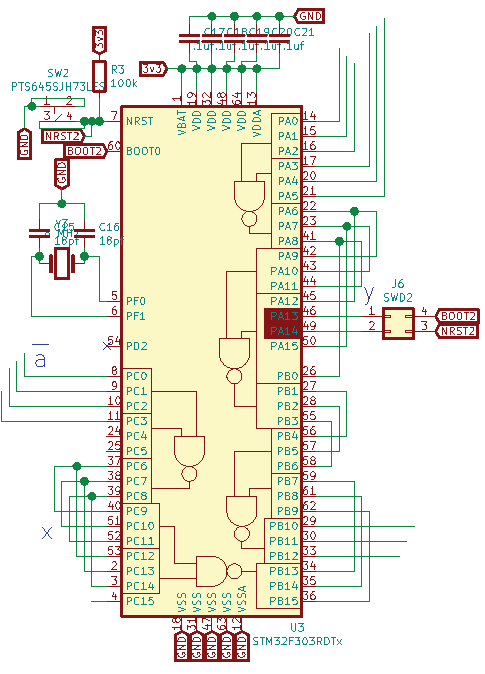
\includegraphics[width=0.95 \linewidth]{chip}
  \caption{The STM32F303RDT6 wired up as 5 {\tt NAN} gates, shown here
    {\it in situ}. This is a portion of a larger schematic.
    Also shown is some support hardware needed for each microprocessor:
    A programming header, 5 filter capacitors, a crystal oscillator circuit,
    and a reset switch with external pull-up.
  }
  \label{fig:schematic}
  \end{center}
\end{figure}

So now we know that we can build arbitrary computers with the {\tt
  NAN} gate, representing the interconnects between the gates efficiently
with binary3-coded real numbers. All that remains is an efficient
implementation of the {\tt NAN} gate itself. We could emulate such
a thing in software, but software is much slower than hardware;
we would also like to maximize the number of times that we can flip
between states of the gate (the flip FLOPS) per second.

Fortunately, there are several pieces of hardware that implement
IEEE 754 real numbers. I found a moderately-priced micrprocessor
(\$6.48/ea.), the STM32F303RDT6. This is a 32-bit ARM Cortex M4F
processor with hardware floating-point running at 72MHz~\cite{stm32}.
In the rather-difficult-to-solder 10mm surface-mount LQFP64 package,
it has 64 pins, 51 of which can be used for general-purpose IO.
Since a {\tt NAN} gate using the binary3 representation needs 9
pins ($3 \times 2$ for the inputs, $3$ for the outputs), it is
feasible to implement five {\tt NAN} gates on the same chip with
a few pins left over for jiggery pokery (Figure~\ref{fig:schematic}).

\begin{figure*}[t!]
  \begin{center}
    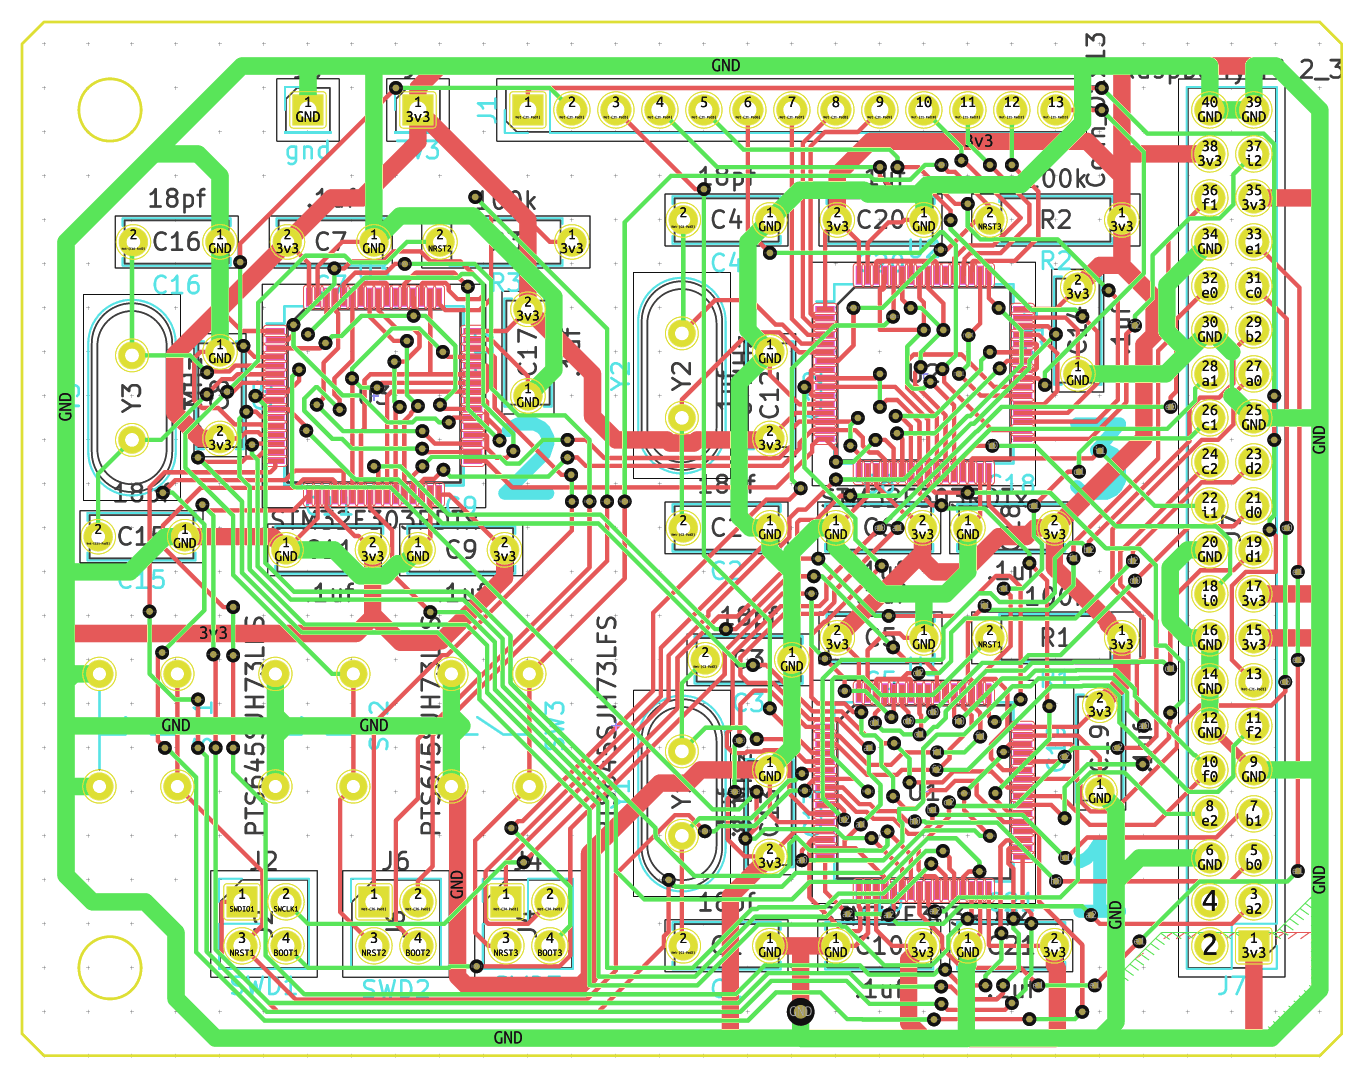
\includegraphics[width=0.55 \linewidth]{board}
  \end{center}\vspace{-0.1in}
  \caption{A beautiful hand-routed circuit board implementing a
    universal math accelerator, using only the universal {\tt NAN} gate
    implemented with native floating point hardware.}
  \label{fig:board}
\end{figure*}

The hardware math accelerator itself can be thought of as a floating
point unit (FPU), but one that is streamlined to run only a single
instruction, the universal function $\inf - {\tt maxNum}(a + b, -\inf)$.
This is a function taking two binary3 real numbers and
outputting a single binary3 number. Since there are only $2^6 = 64$
possible inputs, it can be straightforwardly implemented with table
lookup, but this would require dozens of microprocessors, which
might exceed our power budget. In fact there is significant structure
to the function; for one thing, it can only return $\nan$ or $\inf$ (even
if arguments like -1.0 or 0.0 are given), and the
binary3 representation of these only differ in one bit. Equivalent
logic to determine that bit is as follows:

\begin{small}
\begin{code}
if isfinite(a) && isfinite(b)
then
  // inf - (a + b) = inf
  0
else
  // a + b is nan when a is nan, b is nan, or a and b are
  // infinites with different signs. If they are both
  // -inf, then we have max(-inf, -inf) anyway, which is
  // the same as max(nan, -inf). So we have:
  if a == inf && b == inf
    // both positive infinities
    // inf - inf = nan
    1
  else
    // inf - -inf = inf
    0
\end{code}
\end{small}    

So ultimately this function only returns 1 in the case that both
inputs are exactly $+\inf$, the pattern {\tt 0 1 0}.

If the inputs are a0 a1 a2, b0, b1, b2, and outputs
are c0, c1, c2, then:
\begin{small}
\begin{code}
c0 = 0
c1 = 1
c2 = !a0 && !a2 && !b0 && !b2 && a1 && b1
\end{code}
\end{small}

So we can hardwire the outputs c0 and c1, and use the microprocessor-based
{\tt NAN} gates to compute c2 as a small boolean function.

Of course, each $0$ or $1$ above is actually itself a binary3-coded
\nan\ or \inf. Thus on the physical circuit board, this math
accelerator has $2 \times 3 \times 3$ input pins and $1 \times 3
\times 3$ output pins. This is just shy of the total number of IO pins
on the Raspberry~Pi, so we use such a computer to drive the math
accelerator. Given the large number of traces and small footprint of
the microprocessors, routing the board gets somewhat involved
(Figure~\ref{fig:board}).

As of the SIGBOVIK 2019 deadline, such a circuit board has been
manufactured in China and is in possession of the author (actually the
minimum order quantity of 10), but he is somewhat nervous about his
ability to hand-solder these 0.1mm surface-mount leads, so we'll see
how it goes! Please see \url{http://tom7.org/nan} for project updates
or an embarrassing {\tt 404 Not Found} if I fail to reboot computing
using the beautiful foundation of real numbers.

\bibliography{nand}{}
\bibliographystyle{plain}

\end{document}
